\documentclass[en,12pt,mtpro2]{elegantpaper}

\title{Notes: Double/Debiased Machine Learning}
\author{Ziyang Gong}
\date{}

\usepackage{subcaption, amssymb}

\begin{document}

\maketitle

% \section{Intution}

% \subsection{Regularization Bias}

% \begin{enumerate}
%     \item Non Orthogonal: Suppose $\hat{g}$ are estimated using the auxiliary samples indexed by $\mathrm{I}^{c}$, thus
%           \begin{equation}
%               \check{\theta}=\left(\frac{1}{n}\sum_{i\in\mathrm{I}}D_{i}^{2}\right)^{-1}\frac{1}{n}\sum_{i\in\mathrm{I}}D_{i}\left(Y_{i}-\hat{g}\left(X_{i}\right)\right)
%           \end{equation}
%     \item Orthogonal:  Suppose $\hat{g}$ and $\hat{m}$ are estimated using the auxiliary samples indexed by $\mathrm{I}^{c}$, thus
%           \begin{equation}
%               \check{\theta}=\left(\frac{1}{n}\sum_{i\in\mathrm{I}}\widehat{V}_{i}D_{i}\right)^{-1}\frac{1}{n}\sum_{i\in\mathrm{I}}\hat{V}_{i}\left(Y_{i}-\hat{g}\left(X_{i}\right)\right)
%           \end{equation}
%           where $\hat{V}=D-\hat{m}(\mathbf{X})$.
% \end{enumerate}

% \begin{figure}[htp]
%     \centering
%     \begin{subfigure}{.415\textwidth}
%         \centering
%         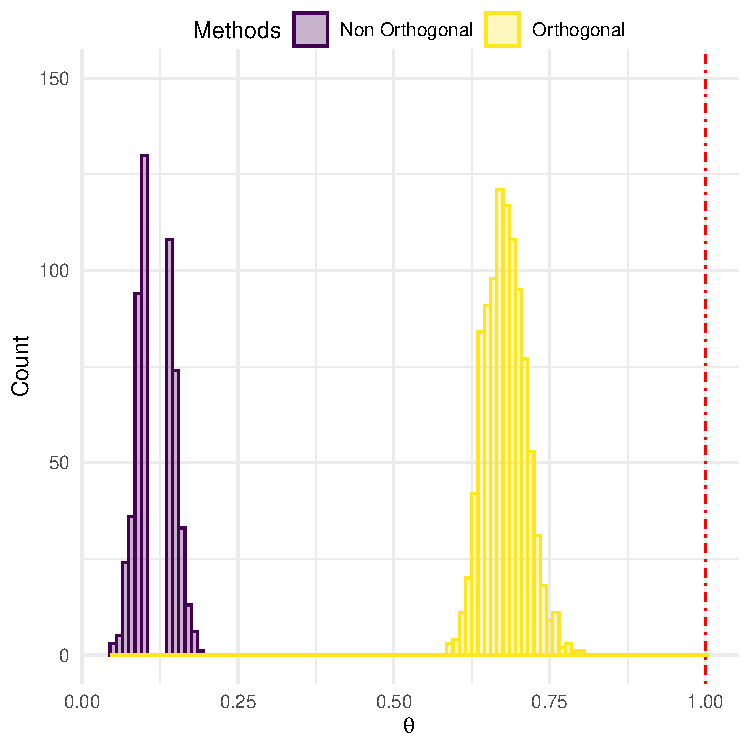
\includegraphics[width=\linewidth]{figures/intution-non-orthogonal-vs-orthogonal-lasso.pdf}
%         \caption{LASSO}
%     \end{subfigure}
%     \begin{subfigure}{.415\textwidth}
%         \centering
%         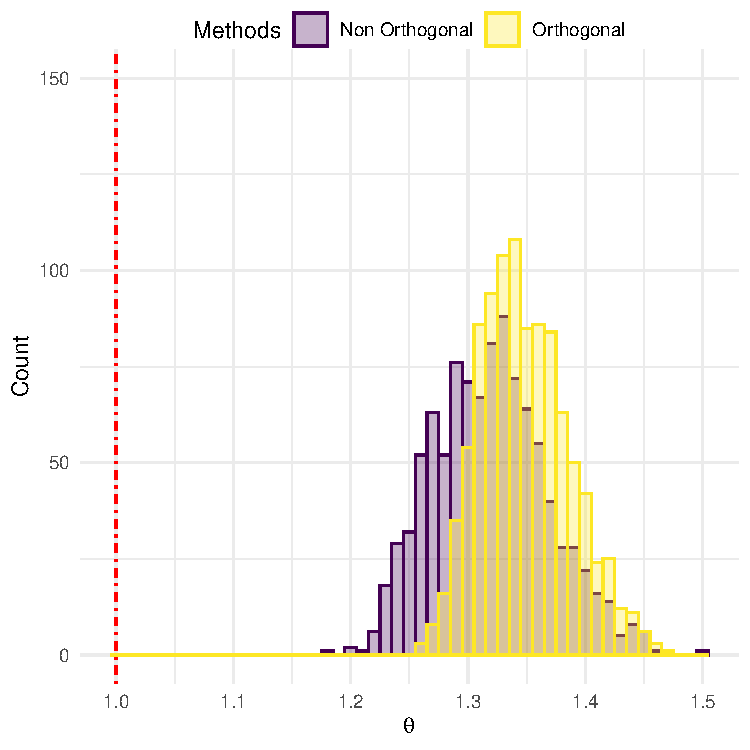
\includegraphics[width=\linewidth]{figures/intution-non-orthogonal-vs-orthogonal-rf.pdf}
%         \caption{Random Forest}
%     \end{subfigure}
%     \caption{Bias Raised by Regularization of Machine Learning}
% \end{figure}

% \subsection{Overfitting Bias}

% \begin{figure}[htp]
%     \centering
%     \begin{subfigure}{.415\textwidth}
%         \centering
%         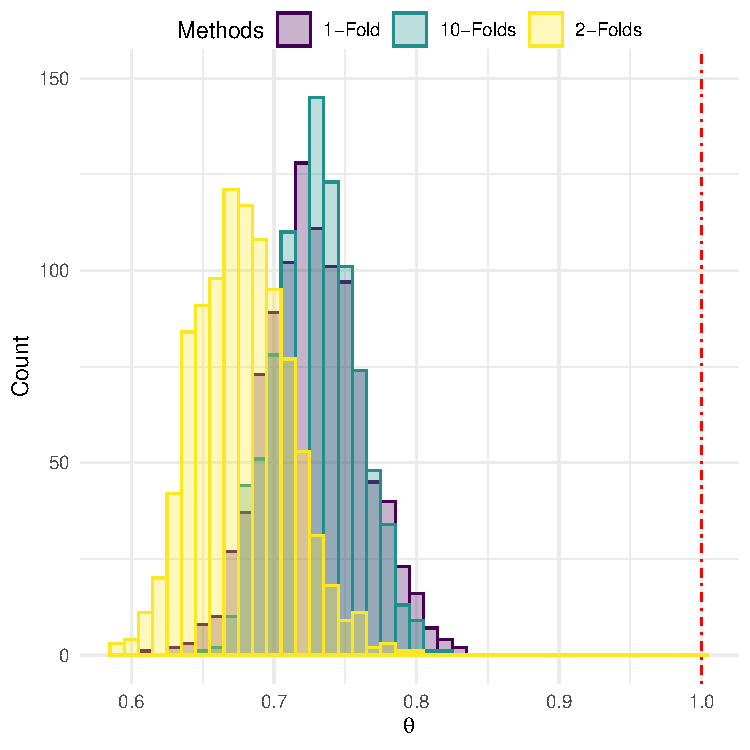
\includegraphics[width=\linewidth]{figures/intution-full-sample-vs-split-sample-lasso.pdf}
%         \caption{LASSO}
%     \end{subfigure}
%     \begin{subfigure}{.415\textwidth}
%         \centering
%         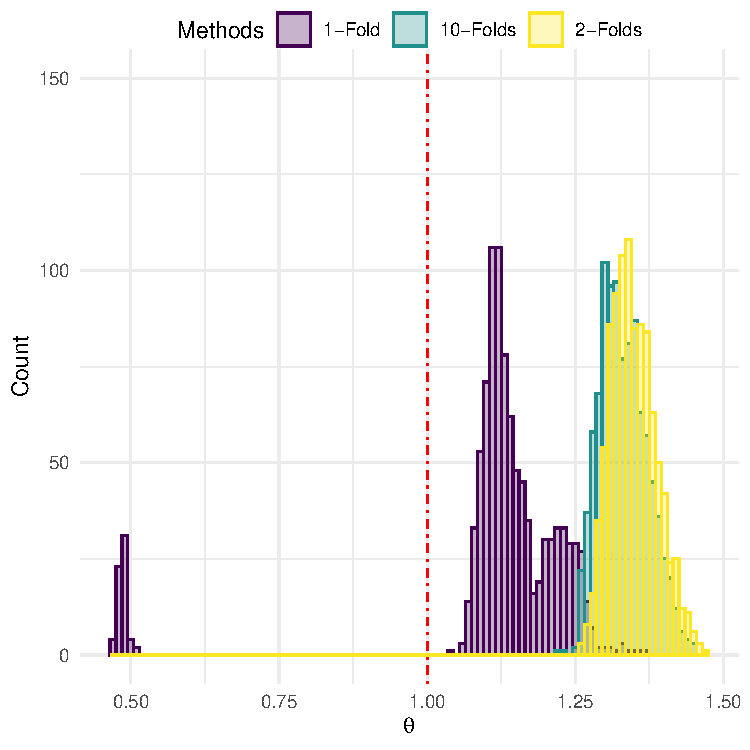
\includegraphics[width=\linewidth]{figures/intution-full-sample-vs-split-sample-rf.pdf}
%         \caption{Random Forest}
%     \end{subfigure}
%     \caption{Bias Raised by Overfitting of Machine Learning}
% \end{figure}

% \subsection{Score Functions}

% \begin{enumerate}
%     \item IV-type: The score function of IV-type is
%           \begin{equation}
%               \psi\left(\mathbf{W};\theta,\boldsymbol{\eta}\right):=\left[Y-D\theta-g(\mathbf{X})\right]\left[D-m(\mathbf{X})\right]
%           \end{equation}
%           where $\boldsymbol{\eta}=(g,m)$. Suppose $\hat{g}$ and $\hat{m}$ are estimated using the auxiliary samples indexed by $\mathrm{I}^{c}$, Thus
%           \begin{equation}
%               \check{\theta}=\left(\frac{1}{n}\sum_{i\in\mathrm{I}}\widehat{V}_{i}D_{i}\right)^{-1}\frac{1}{n}\sum_{i\in\mathrm{I}}\hat{V}_{i}\left(Y_{i}-\hat{g}\left(X_{i}\right)\right)
%           \end{equation}
%           where $\hat{V}=D-\hat{m}(\mathbf{X})$.
%     \item Partialling-Out: The score function of partialling-out is
%           \begin{equation}
%               \psi\left(\mathbf{W};\theta,\boldsymbol{\eta}\right):=\left[Y-\ell\left(\mathbf{X})-\theta\left(D-m(\mathbf{X}\right)\right)\right]\left[D-m(\mathbf{X})\right]
%           \end{equation}
%           where $\boldsymbol{\eta}=(\ell,m)$. Suppose $\hat{\ell}$ and $\hat{m}$ are estimated using the auxiliary samples indexed by $\mathrm{I}^{c}$, Thus
%           \begin{equation}
%               \check{\theta}=\left(\frac{1}{n}\sum_{i\in\mathrm{I}}\widehat{V}_{i}^{2}\right)^{-1}\frac{1}{n}\sum_{i\in\mathrm{I}}\hat{V}_{i}\left(Y_{i}-\hat{\ell}\left(X_{i}\right)\right)
%           \end{equation}
%           where $\hat{V}=D-\hat{m}(\mathbf{X})$.
% \end{enumerate}

% \begin{figure}[htp]
%     \centering
%     \begin{subfigure}{.415\textwidth}
%         \centering
%         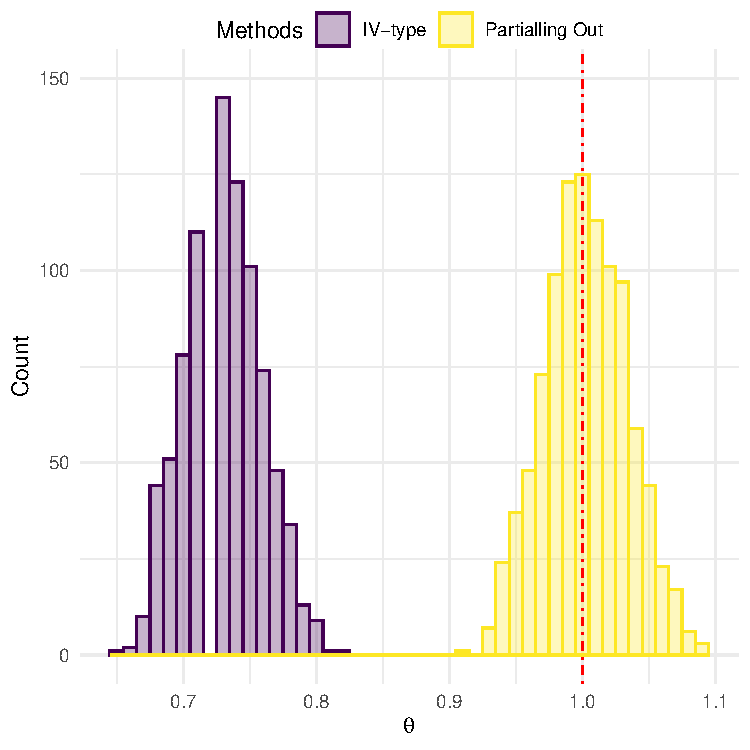
\includegraphics[width=\linewidth]{figures/intution-iv-type-vs-partialling-out-lasso.pdf}
%         \caption{LASSO}
%     \end{subfigure}
%     \begin{subfigure}{.415\textwidth}
%         \centering
%         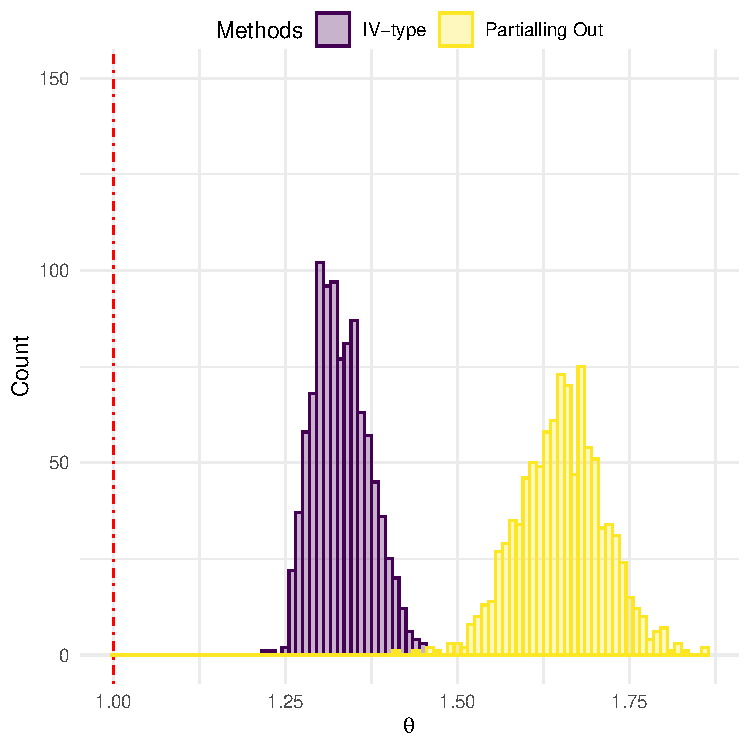
\includegraphics[width=\linewidth]{figures/intution-iv-type-vs-partialling-out-rf.pdf}
%         \caption{Random Forest}
%     \end{subfigure}
%     \caption{Bias Raised by Score Functions}
% \end{figure}

% \subsection{Complexity of Paramters}

% \begin{figure}[htp]
%     \centering
%     \begin{subfigure}{.415\textwidth}
%         \centering
%         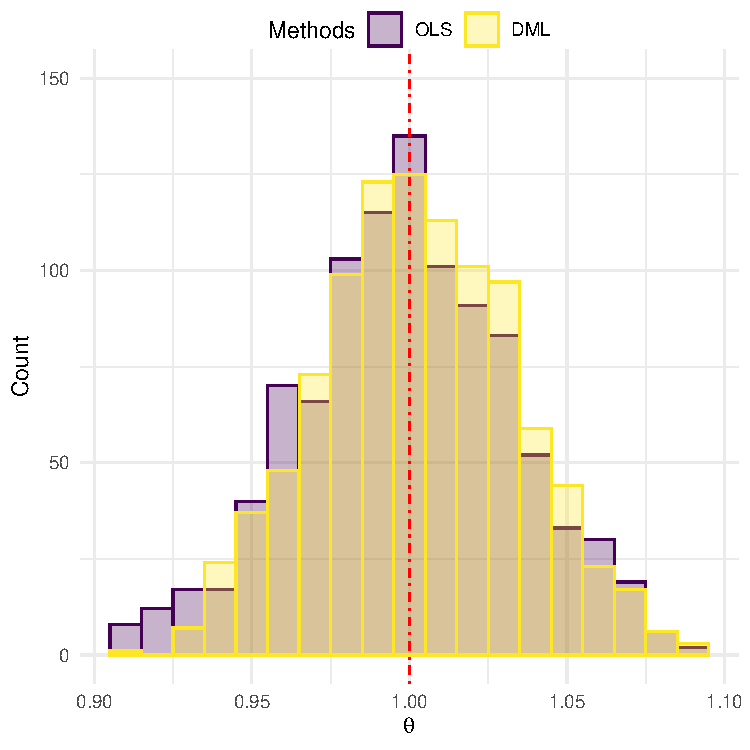
\includegraphics[width=\linewidth]{figures/intution-ols-vs-dml-lasso.pdf}
%         \caption{LASSO}
%     \end{subfigure}
%     \begin{subfigure}{.415\textwidth}
%         \centering
%         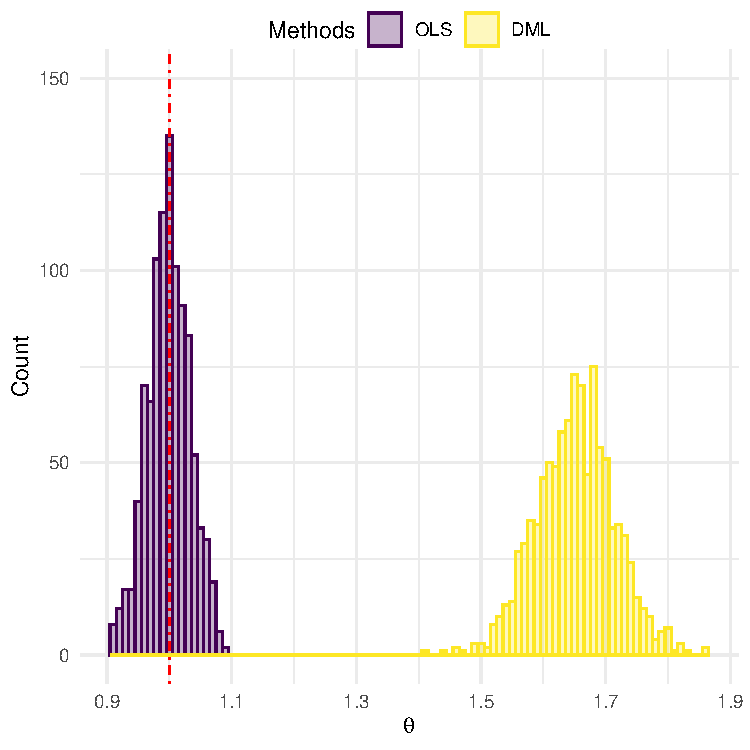
\includegraphics[width=\linewidth]{figures/intution-ols-vs-dml-rf.pdf}
%         \caption{Random Forest}
%     \end{subfigure}
%     \caption{Bias and Heterogeneity Raised by Complexity of Paramters}
% \end{figure}

Consider the partical linear regression model
\begin{equation}
    \begin{aligned}
        Y_{i}=D_{i}\theta+g(\mathbf{X}_{i})+U_{i}, & \quad E\left(U_{i}\mid\mathbf{X}_{i},D_{i}\right)=0 \\
        D_{i}=m(\mathbf{X}_{i})+V_{i},             & \quad E\left(V_{i}\mid\mathbf{X}_{i}\right)=0
    \end{aligned}
\end{equation}
where $\mathbf{X}_{i}\in\mathbb{R}^{p}$, $i=1,2,\ldots,n$.

Consider the following score functions for partical linear regression, that,
\begin{enumerate}
    \item IV-type: The score function of IV-type is
          \begin{equation}
              \psi\left(\mathbf{W};\theta,\boldsymbol{\eta}\right):=\left[Y-D\theta-g(\mathbf{X})\right]\left[D-m(\mathbf{X})\right]
          \end{equation}
          where $\boldsymbol{\eta}=(g,m)$. Suppose $\hat{g}$ and $\hat{m}$ are estimated using the auxiliary samples indexed by $\mathrm{I}^{c}$, Thus
          \begin{equation}
              \check{\theta}=\left(\frac{1}{n}\sum_{i\in\mathrm{I}}\widehat{V}_{i}D_{i}\right)^{-1}\frac{1}{n}\sum_{i\in\mathrm{I}}\hat{V}_{i}\left(Y_{i}-\hat{g}\left(X_{i}\right)\right)
          \end{equation}
          where $\hat{V}=D-\hat{m}(\mathbf{X})$.
    \item Partialling-Out: The score function of partialling-out is
          \begin{equation}
              \psi\left(\mathbf{W};\theta,\boldsymbol{\eta}\right):=\left[Y-\ell\left(\mathbf{X})-\theta\left(D-m(\mathbf{X}\right)\right)\right]\left[D-m(\mathbf{X})\right]
          \end{equation}
          where $\boldsymbol{\eta}=(\ell,m)$. Suppose $\hat{\ell}$ and $\hat{m}$ are estimated using the auxiliary samples indexed by $\mathrm{I}^{c}$, Thus
          \begin{equation}
              \check{\theta}=\left(\frac{1}{n}\sum_{i\in\mathrm{I}}\widehat{V}_{i}^{2}\right)^{-1}\frac{1}{n}\sum_{i\in\mathrm{I}}\hat{V}_{i}\left(Y_{i}-\hat{\ell}\left(X_{i}\right)\right)
          \end{equation}
          where $\hat{V}=D-\hat{m}(\mathbf{X})$.
\end{enumerate}

In this note, we use samples $n=200$ and repeat 1000 times to evaluate the estimation effects of different models, and the code is avaliable at \href{https://github.com/SignorinoY/ultralisk}{https://github.com/SignorinoY/ultralisk}.
\clearpage

\section{Linear Models}

Suppose
\begin{equation}
    \begin{array}{cc}
        m(\mathbf{X}_{i})=\sum_{j=1}^{3}\alpha_{j}x_{i,j},\quad g(\mathbf{X}_{i})=\sum_{j=1}^{3}\beta_{j}x_{i,j} \\
        \boldsymbol{\alpha}=\left(3,2,1\right)^{\prime},\quad\boldsymbol{\beta}=\left(1,2,3\right)^{\prime}
    \end{array}
    \label{eq:linear-model-1}
\end{equation}
or
\begin{equation}
    \begin{array}{cc}
        m(\mathbf{X}_{i})=\sum_{j=1}^{6}\alpha_{j}x_{i,j},\quad g(\mathbf{X}_{i})=\sum_{j=1}^{6}\beta_{j}x_{i,j} \\
        \boldsymbol{\alpha}=\left(6,5,4,3,2,1\right)^{\prime},\quad\boldsymbol{\beta}=\left(1,2,3,4,5,6\right)^{\prime}
    \end{array}
    \label{eq:linear-model-2}
\end{equation}
where
\begin{equation*}
    \mathbf{X}_{i}\sim N\left(\boldsymbol{0},\mathrm{I}_{p}\right)\text{ and }U_{i},V_{i}\sim N\left(0,1\right),\quad i=1,2,\ldots,n.
\end{equation*}

\begin{figure}[htp]
    \centering
    \begin{subfigure}{.41\textwidth}
        \centering
        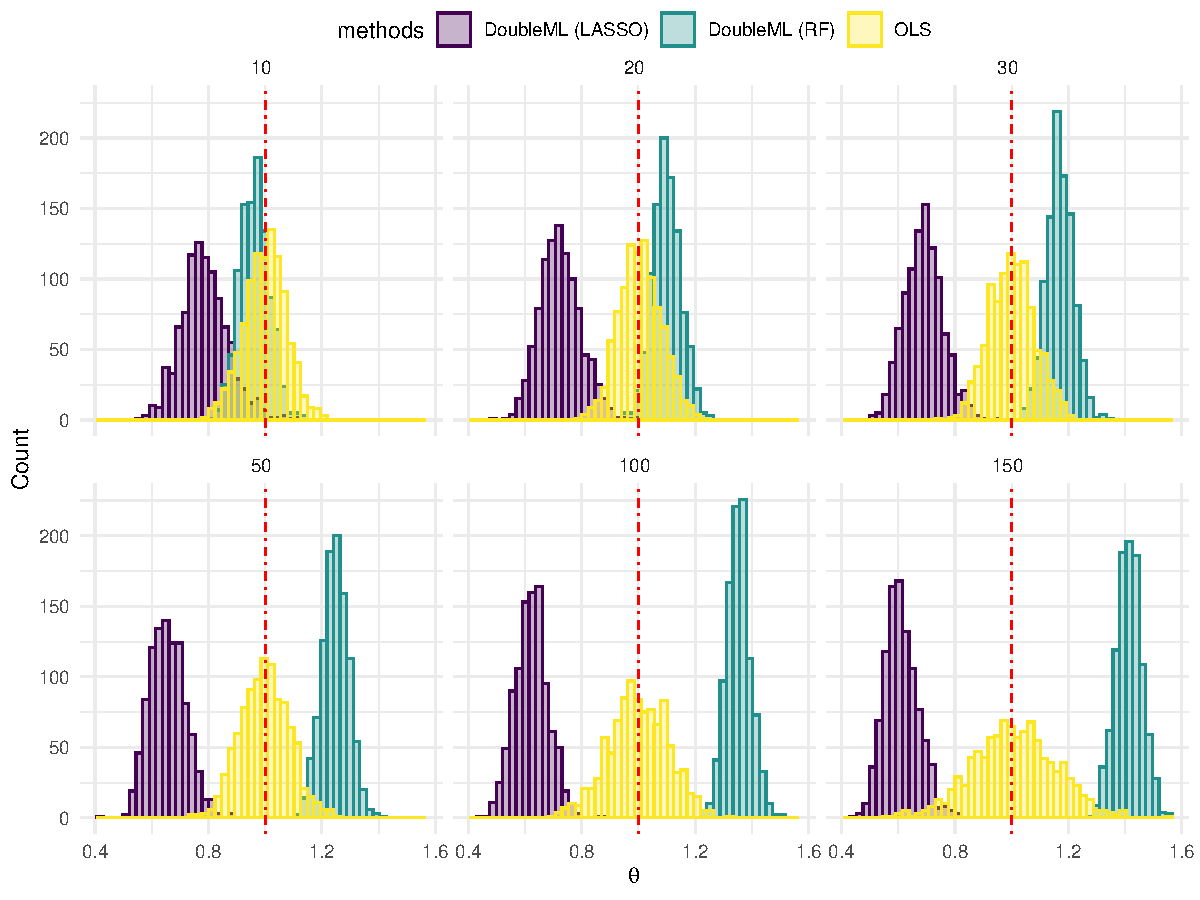
\includegraphics[width=\linewidth]{figures/simulation-linear3 (IV-type).pdf}
        \caption{IV-type}
    \end{subfigure}
    \begin{subfigure}{.41\textwidth}
        \centering
        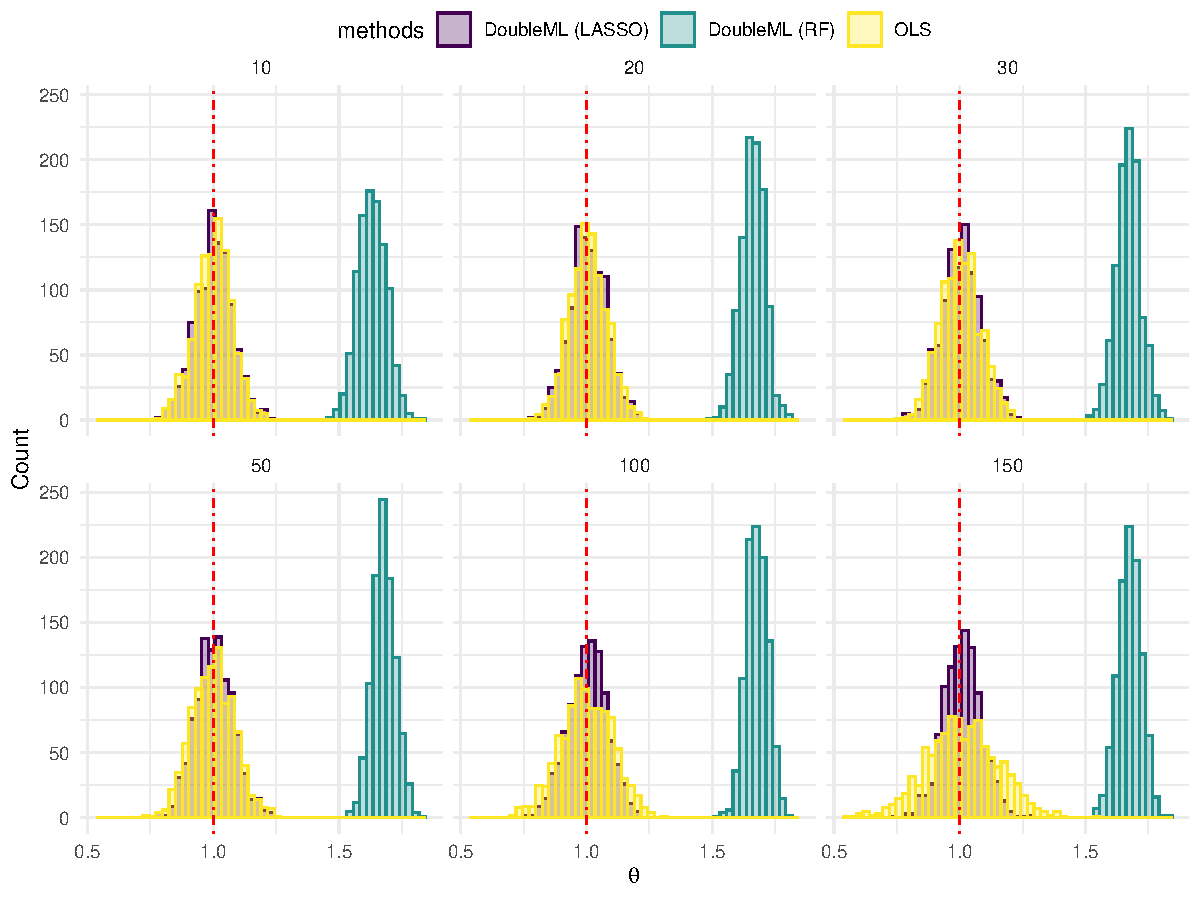
\includegraphics[width=\linewidth]{figures/simulation-linear3 (partialling out).pdf}
        \caption{Partialling-Out}
    \end{subfigure}
    \caption{Linear Models for (\ref{eq:linear-model-1})}
\end{figure}

\begin{figure}[htp]
    \centering
    \begin{subfigure}{.41\textwidth}
        \centering
        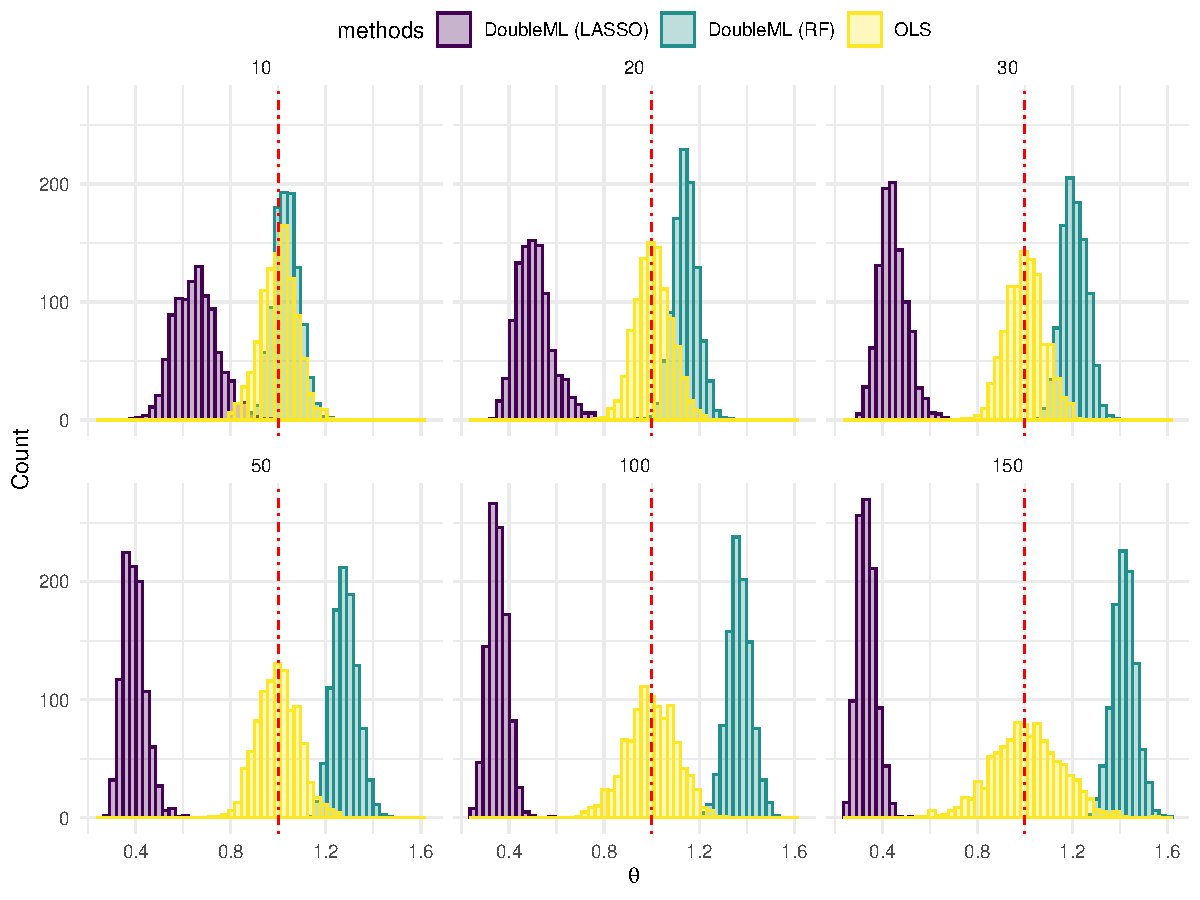
\includegraphics[width=\linewidth]{figures/simulation-linear6 (IV-type).pdf}
        \caption{IV-type}
    \end{subfigure}
    \begin{subfigure}{.41\textwidth}
        \centering
        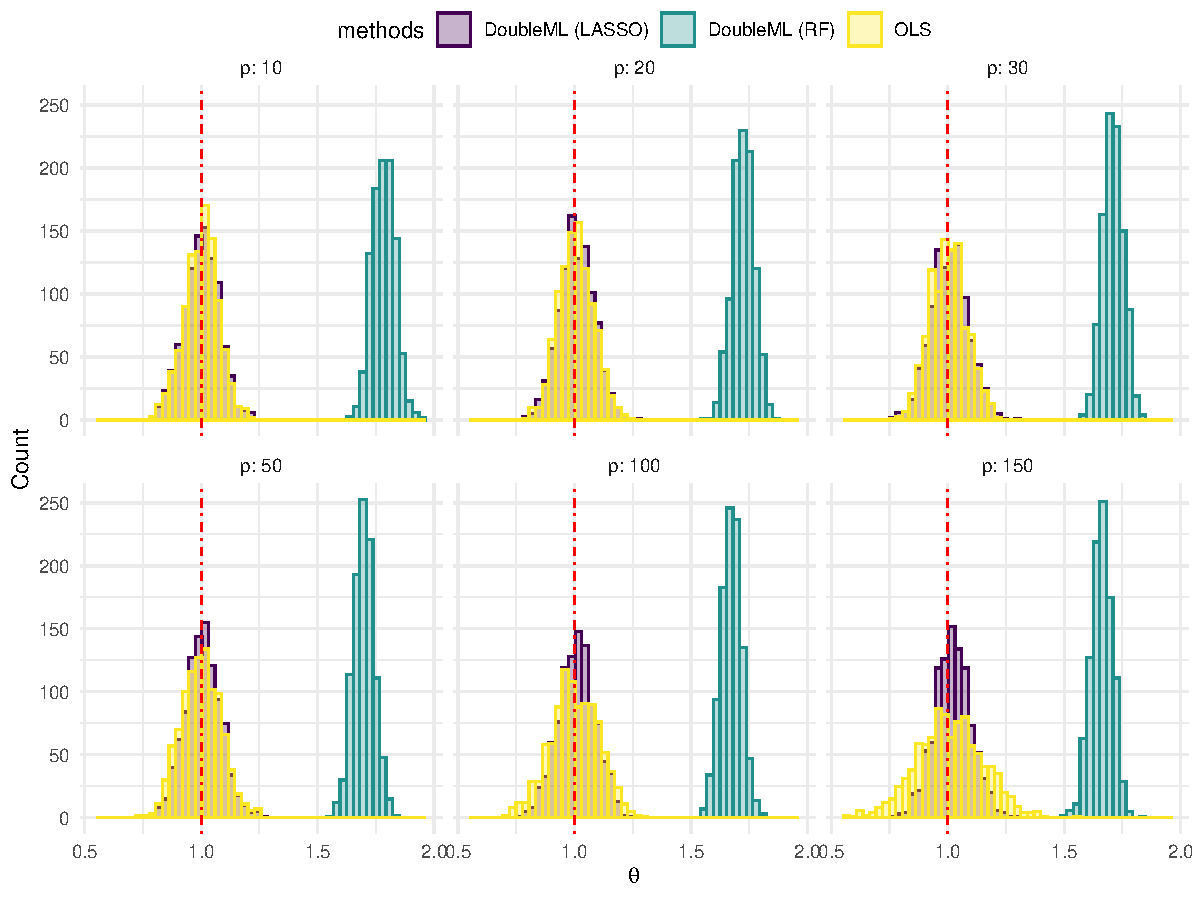
\includegraphics[width=\linewidth]{figures/simulation-linear6 (partialling out).pdf}
        \caption{Partialling-Out}
    \end{subfigure}
    \caption{Linear Models for (\ref{eq:linear-model-2})}
\end{figure}
\clearpage

\section{Relu Models}

Suppose
\begin{equation}
    \begin{array}{cc}
        m(\mathbf{X}_{i})=\sum_{j=1}^{3}\alpha_{j}\max\left(x_{i,j},0\right),\quad g(\mathbf{X}_{i})=\sum_{j=1}^{3}\beta_{j}\max\left(x_{i,j},0\right) \\
        \boldsymbol{\alpha}=\left(3,2,1\right)^{\prime},\quad\boldsymbol{\beta}=\left(1,2,3\right)^{\prime}
    \end{array}
    \label{eq:relu-model-1}
\end{equation}
or
\begin{equation}
    \begin{array}{cc}
        m(\mathbf{X}_{i})=\sum_{j=1}^{6}\alpha_{j}\max\left(x_{i,j},0\right),\quad g(\mathbf{X}_{i})=\sum_{j=1}^{6}\beta_{j}\max\left(x_{i,j},0\right) \\
        \boldsymbol{\alpha}=\left(6,5,4,3,2,1\right)^{\prime},\quad\boldsymbol{\beta}=\left(1,2,3,4,5,6\right)^{\prime}
    \end{array}
    \label{eq:relu-model-2}
\end{equation}
where
\begin{equation*}
    \mathbf{X}_{i}\sim N\left(\boldsymbol{0},\mathrm{I}_{p}\right)\text{ and }U_{i},V_{i}\sim N\left(0,1\right),\quad i=1,2,\ldots,n.
\end{equation*}

\begin{figure}[htp]
    \centering
    \begin{subfigure}{.41\textwidth}
        \centering
        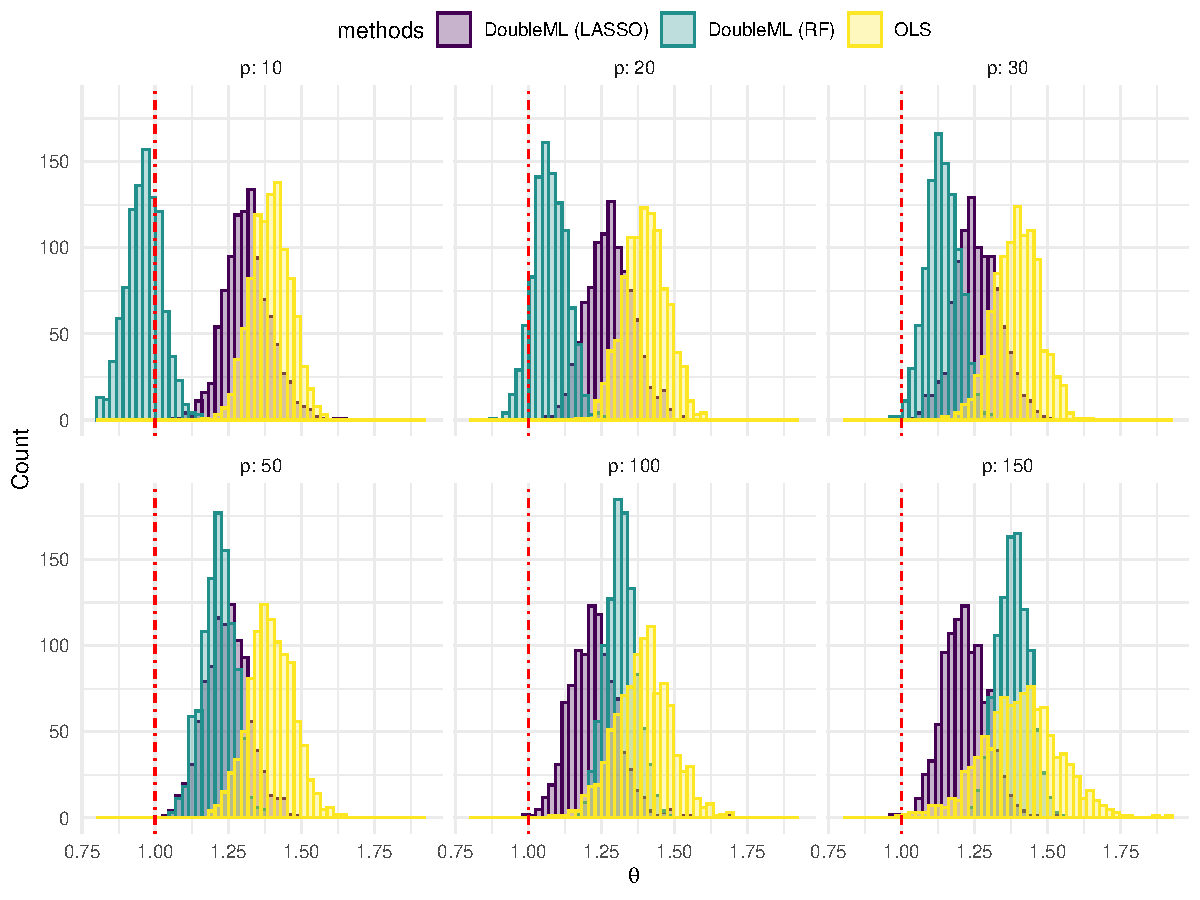
\includegraphics[width=\linewidth]{figures/simulation-relu3 (IV-type).pdf}
        \caption{IV-type}
    \end{subfigure}
    \begin{subfigure}{.41\textwidth}
        \centering
        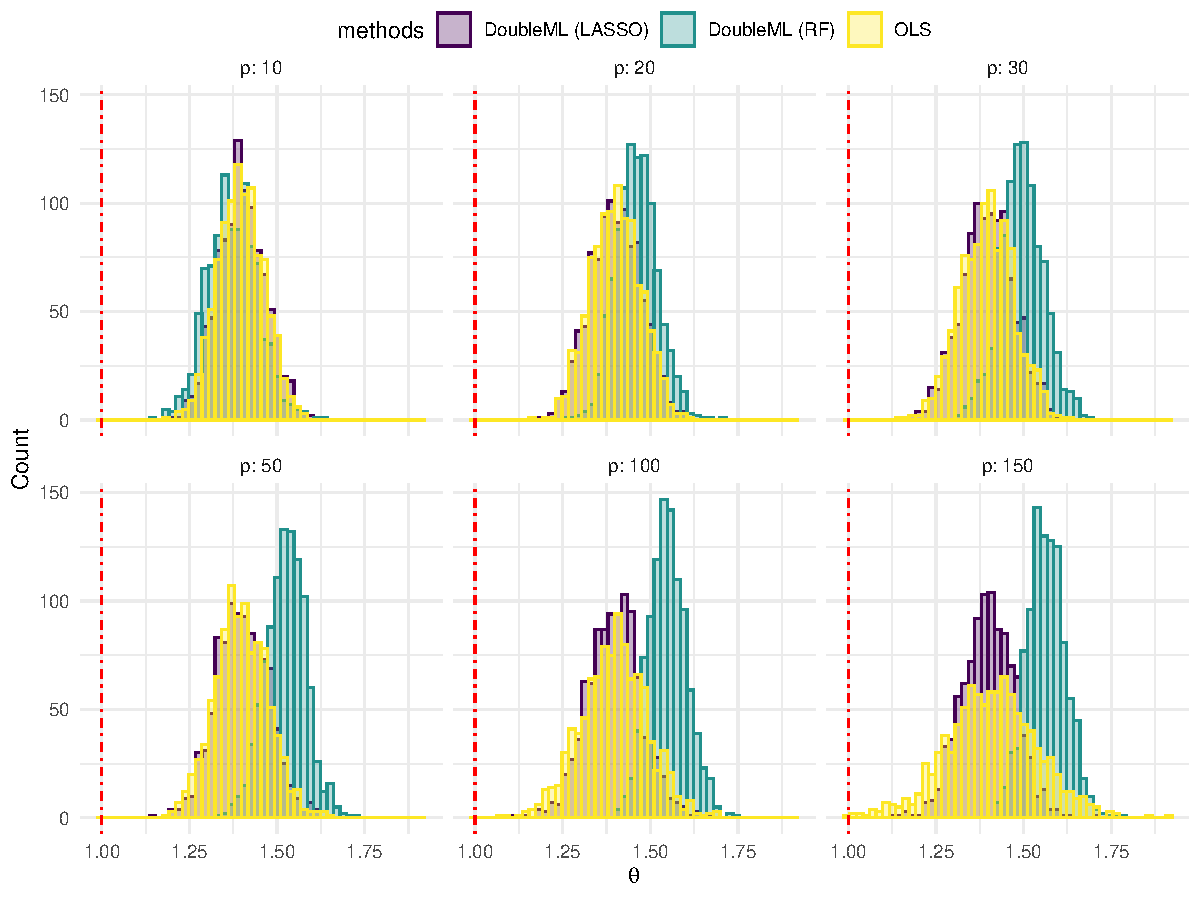
\includegraphics[width=\linewidth]{figures/simulation-relu3 (partialling out).pdf}
        \caption{Partialling-Out}
    \end{subfigure}
    \caption{Relu Models for (\ref{eq:relu-model-1})}
\end{figure}

\begin{figure}[htp]
    \centering
    \begin{subfigure}{.41\textwidth}
        \centering
        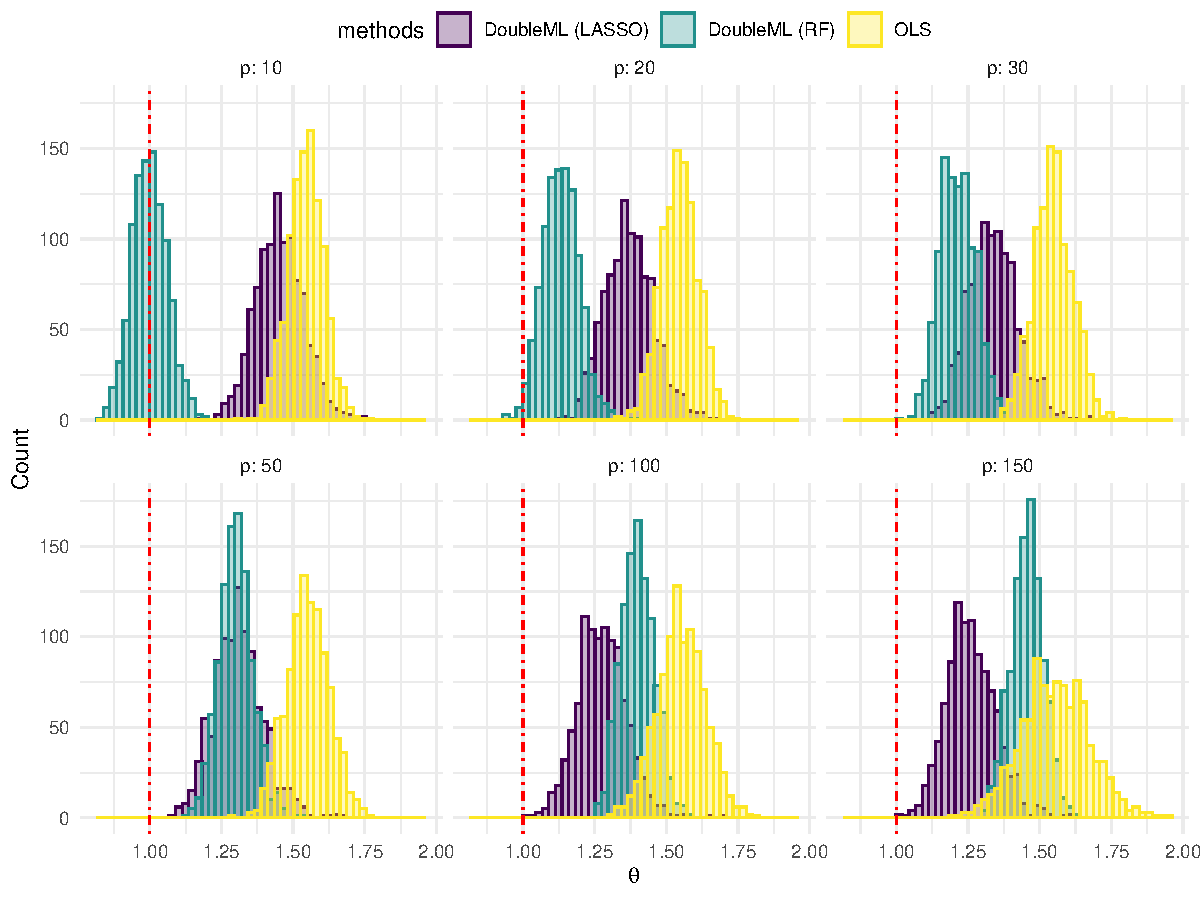
\includegraphics[width=\linewidth]{figures/simulation-relu6 (IV-type).pdf}
        \caption{IV-type}
    \end{subfigure}
    \begin{subfigure}{.41\textwidth}
        \centering
        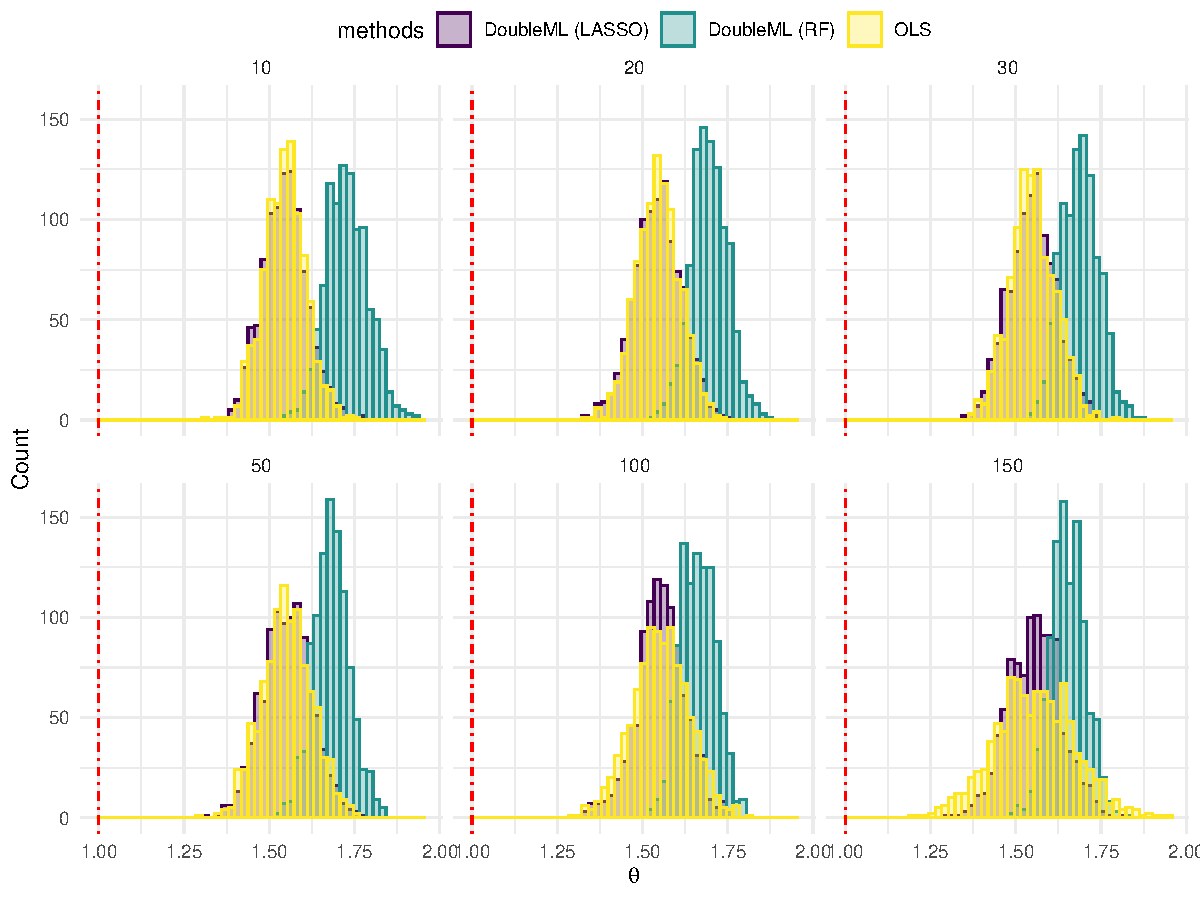
\includegraphics[width=\linewidth]{figures/simulation-relu6 (partialling out).pdf}
        \caption{Partialling-Out}
    \end{subfigure}
    \caption{Relu Models for (\ref{eq:relu-model-2})}
\end{figure}
\clearpage

\section{Polynomial Models}

Suppose
\begin{equation}
    \begin{aligned}
        m(\mathbf{X}_{i})= & x_{i,1}^{3}+x_{i,2}^{2}+x_{i,1}x_{i,2}+x_{i,2}x_{i,3} \\
        g(\mathbf{X}_{i})= & x_{i,2}^{3}+x_{i,3}^{2}+x_{i,1}x_{i,3}+x_{i,2}x_{i,3}
    \end{aligned}
    \label{eq:polynomial-model-1}
\end{equation}
or
\begin{equation}
    m(\mathbf{X}_{i})=\left(\sum_{j=1}^{3}x_{i,j}\right)^{3}+\left(\sum_{j=4}^{6}x_{i,j}\right)^{2},\quad g(\mathbf{X}_{i})=\left(\sum_{j=1}^{3}x_{i,j}\right)^{2}+\left(\sum_{j=4}^{6}x_{i,j}\right)^{3}
    \label{eq:polynomial-model-2}
\end{equation}
where
\begin{equation*}
    \mathbf{X}_{i}\sim N\left(\boldsymbol{0},\mathrm{I}_{p}\right)\text{ and }U_{i},V_{i}\sim N\left(0,1\right),\quad i=1,2,\ldots,n.
\end{equation*}

\begin{figure}[htp]
    \centering
    \begin{subfigure}{.41\textwidth}
        \centering
        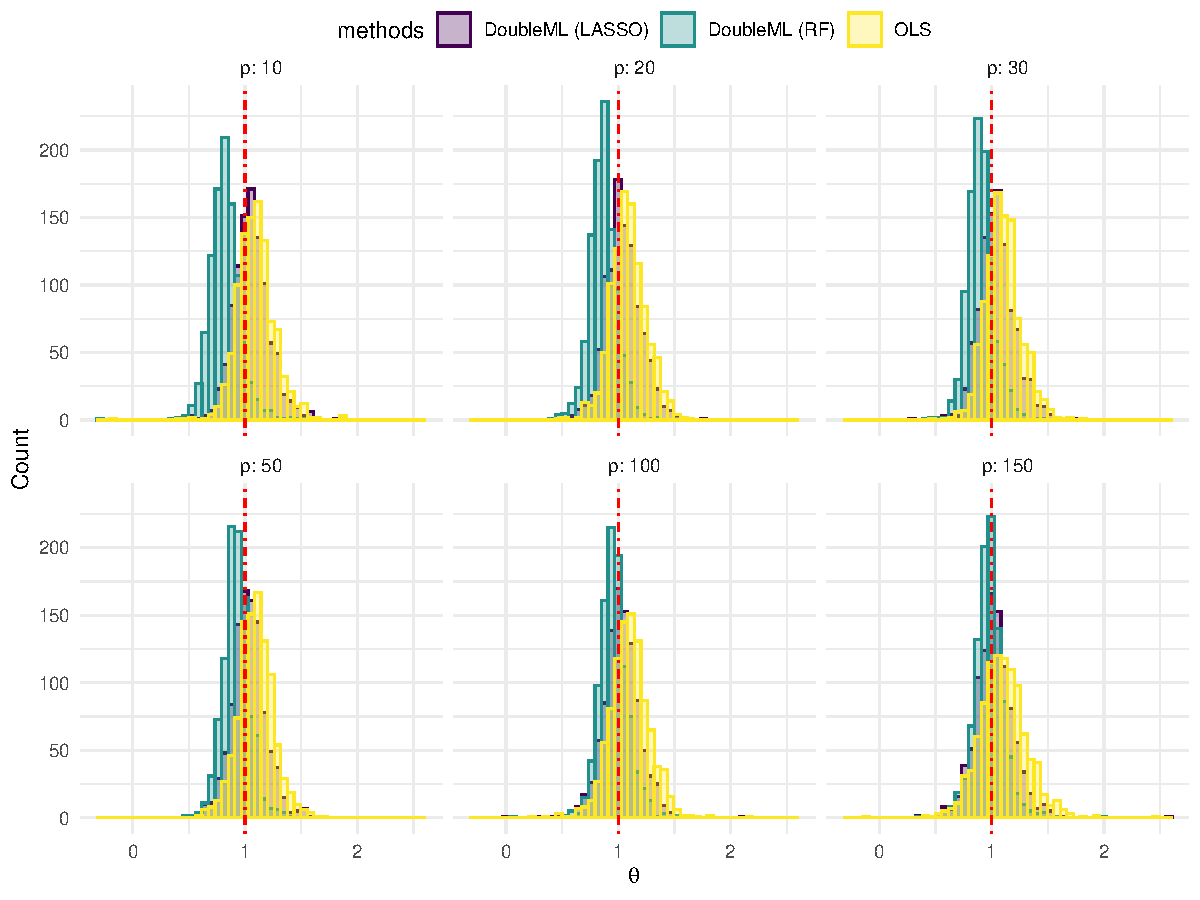
\includegraphics[width=\linewidth]{figures/simulation-polynomial3 (IV-type).pdf}
        \caption{IV-type}
    \end{subfigure}
    \begin{subfigure}{.41\textwidth}
        \centering
        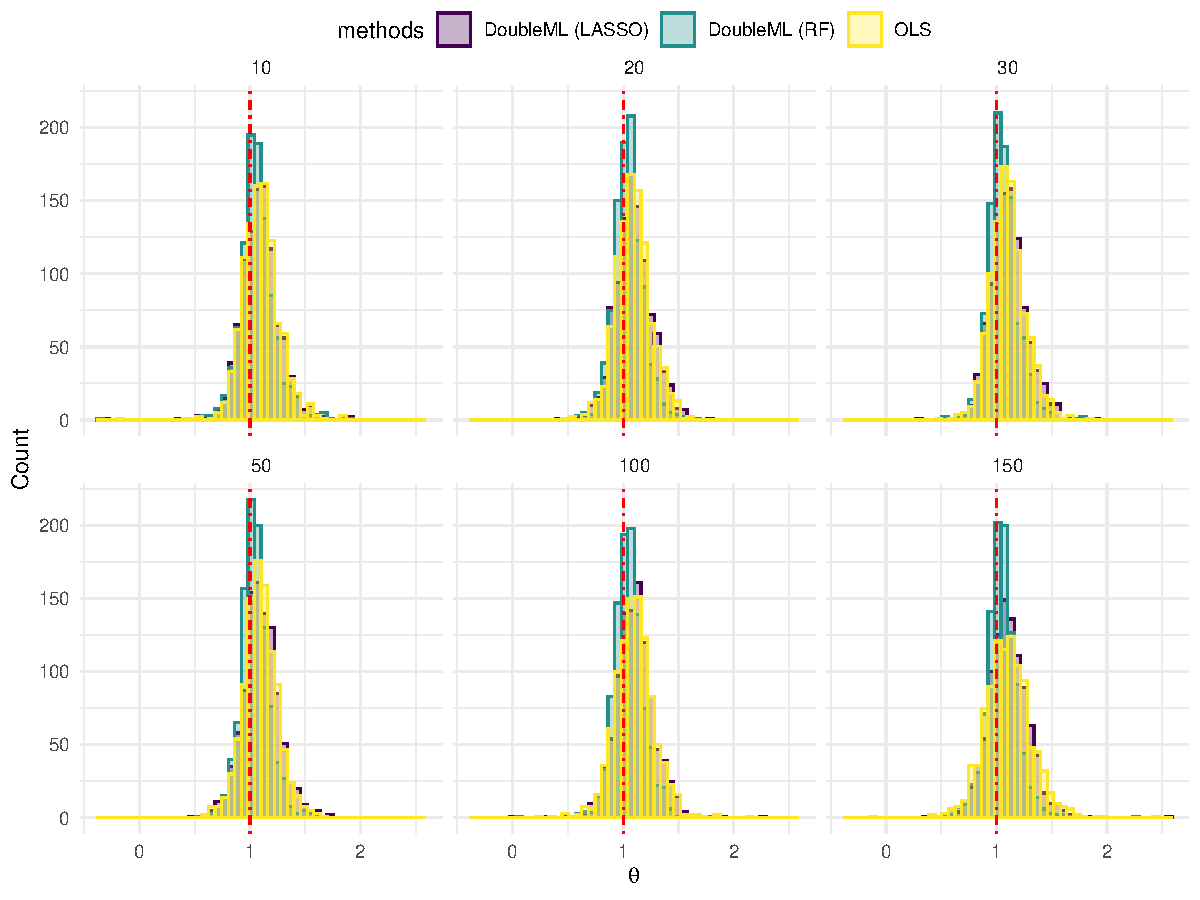
\includegraphics[width=\linewidth]{figures/simulation-polynomial3 (partialling out).pdf}
        \caption{Partialling-Out}
    \end{subfigure}
    \caption{Polynomial Models for (\ref{eq:polynomial-model-1})}
\end{figure}

\begin{figure}[htp]
    \centering
    \begin{subfigure}{.41\textwidth}
        \centering
        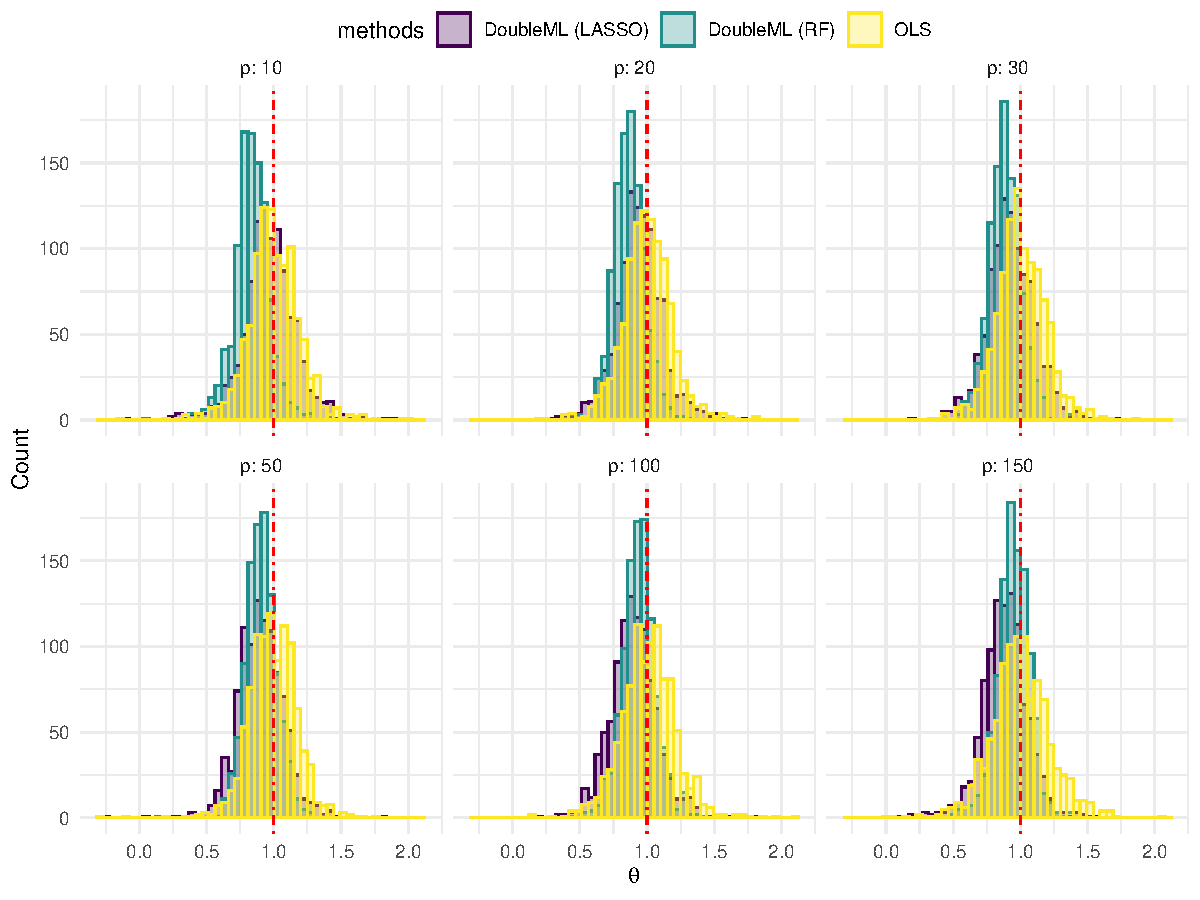
\includegraphics[width=\linewidth]{figures/simulation-polynomial6 (IV-type).pdf}
        \caption{IV-type}
    \end{subfigure}
    \begin{subfigure}{.41\textwidth}
        \centering
        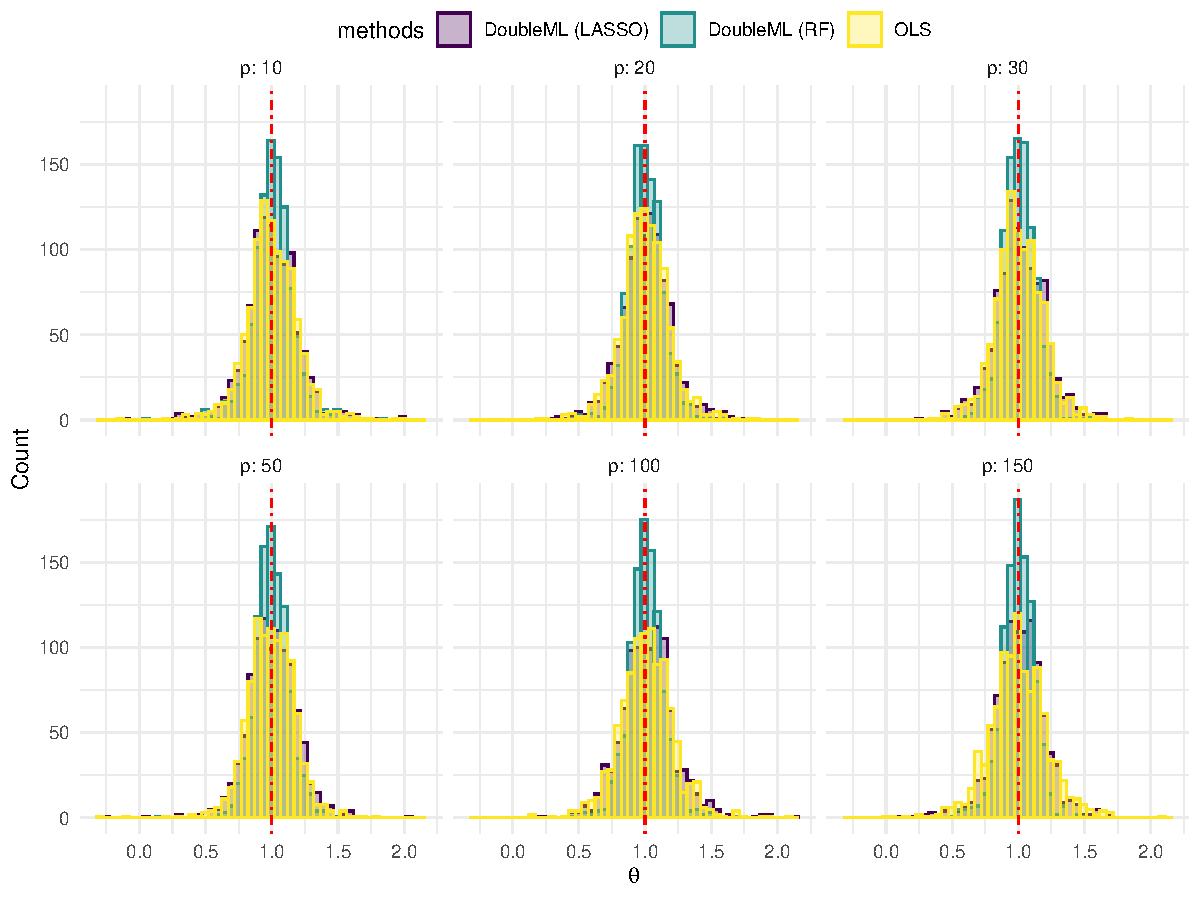
\includegraphics[width=\linewidth]{figures/simulation-polynomial6 (partialling out).pdf}
        \caption{Partialling-Out}
    \end{subfigure}
    \caption{Polynomial Models for (\ref{eq:polynomial-model-2})}
\end{figure}
\clearpage

\section{Logistic-like Models}

Suppose
\begin{equation}
    \begin{aligned}
        m\left(\mathbf{X}_{i}\right)= & \frac{\exp\left(x_{i,1}+x_{i,2}\right)}{1+\exp\left(x_{i,1}+x_{i,2}\right)}+\frac{1}{4}\cdot x_{i,3} \\
        g\left(\mathbf{X}_{i}\right)= & x_{i,1}+\frac{1}{4}\cdot\frac{\exp\left(x_{i,2}+x_{i,3}\right)}{1+\exp\left(x_{i,2}+x_{i,3}\right)}
    \end{aligned}
    \label{eq:logistic-model-1}
\end{equation}
or
\begin{equation}
    \begin{aligned}
        m\left(\mathbf{X}_{i}\right)= & \left[\frac{\exp\left(x_{i,1}+x_{i,2}\right)}{1+\exp\left(x_{i,1}+x_{i,2}\right)}+\frac{\exp\left(x_{i,4}+x_{i,5}\right)}{1+\exp\left(x_{i,4}+x_{i,5}\right)}\right]+\frac{1}{4}\left(x_{i,3}+x_{i,6}\right) \\
        g\left(\mathbf{X}_{i}\right)= & \left(x_{i,1}+x_{i,4}\right)+\frac{1}{4}\left[\frac{\exp\left(x_{i,2}+x_{i,3}\right)}{1+\exp\left(x_{i,2}+x_{i,3}\right)}+\frac{\exp\left(x_{i,5}+x_{i,6}\right)}{1+\exp\left(x_{i,5}+x_{i,6}\right)}\right]
    \end{aligned}
    \label{eq:logistic-model-2}
\end{equation}
where
\begin{equation*}
    \mathbf{X}_{i}\sim N\left(\boldsymbol{0},\mathrm{I}_{p}\right)\text{ and }U_{i},V_{i}\sim N\left(0,1\right),\quad i=1,2,\ldots,n.
\end{equation*}

\begin{figure}[htp]
    \centering
    \begin{subfigure}{.41\textwidth}
        \centering
        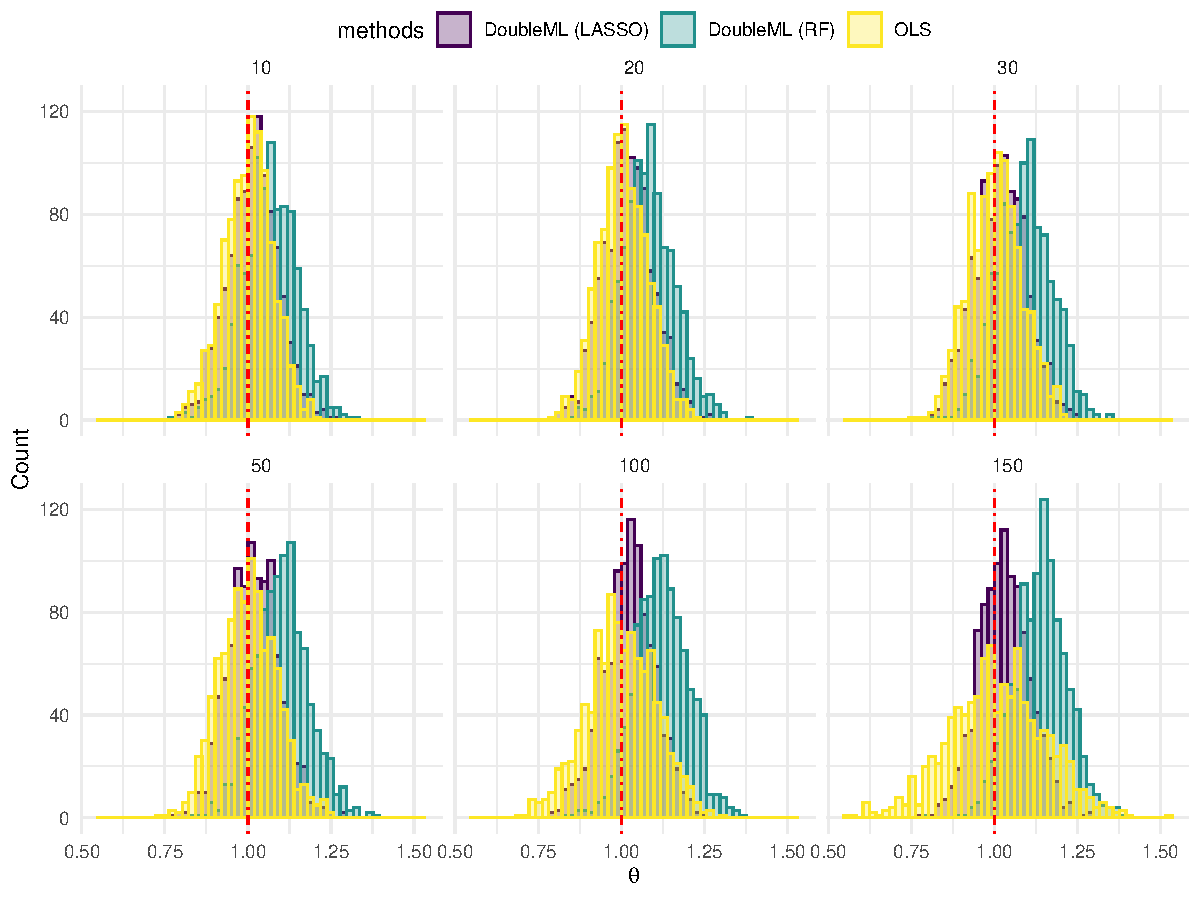
\includegraphics[width=\linewidth]{figures/simulation-logistic3 (IV-type).pdf}
        \caption{IV-type}
    \end{subfigure}
    \begin{subfigure}{.41\textwidth}
        \centering
        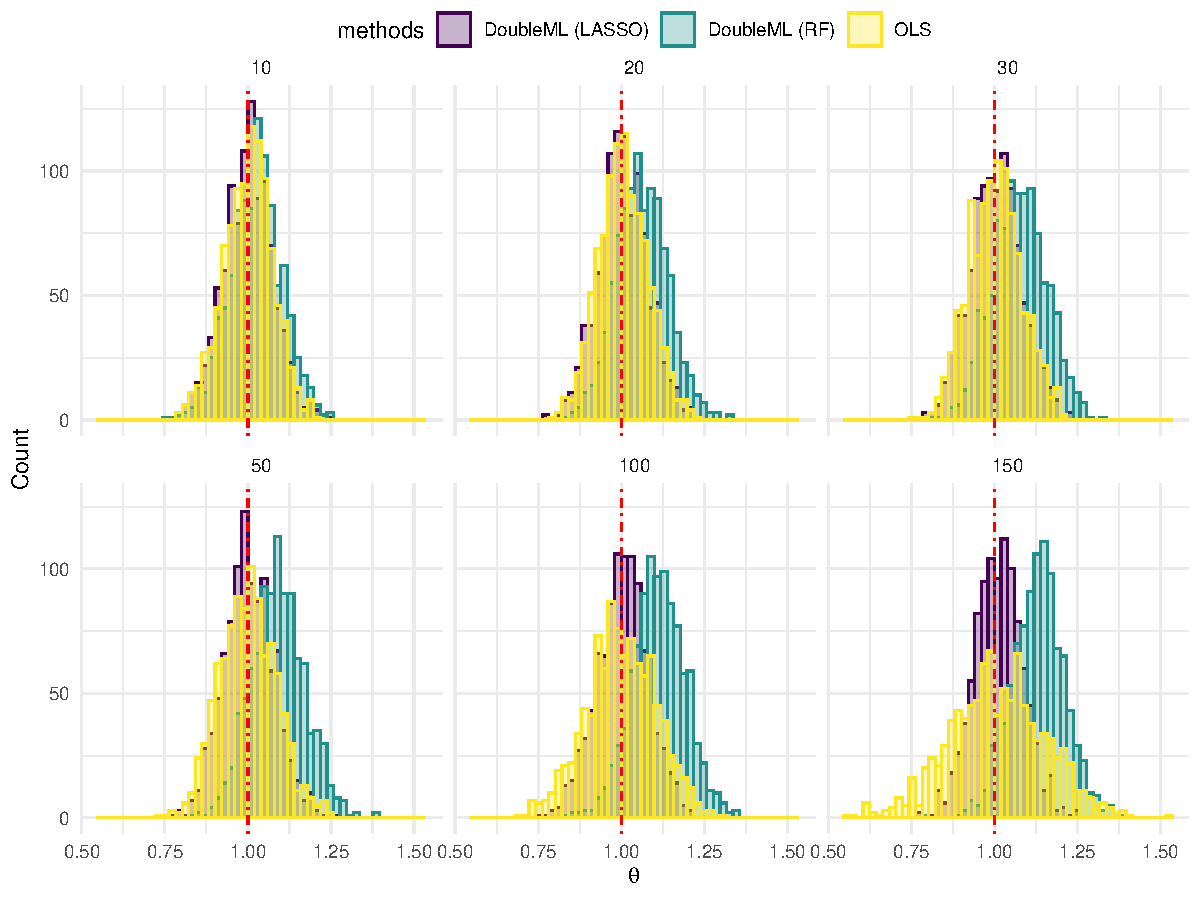
\includegraphics[width=\linewidth]{figures/simulation-logistic3 (partialling out).pdf}
        \caption{Partialling-Out}
    \end{subfigure}
    \caption{Logistic-like Models for (\ref{eq:logistic-model-1})}
\end{figure}

\begin{figure}[htp]
    \centering
    \begin{subfigure}{.41\textwidth}
        \centering
        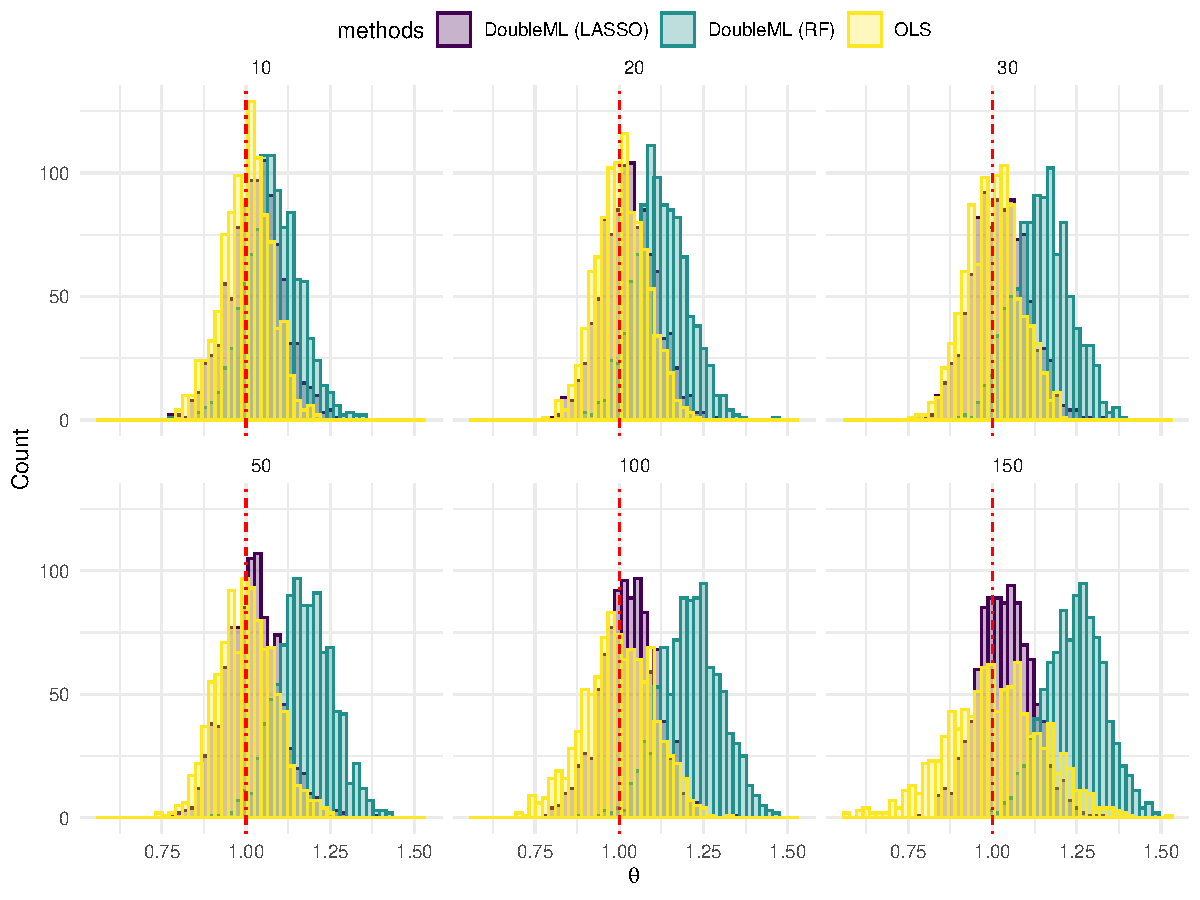
\includegraphics[width=\linewidth]{figures/simulation-logistic6 (IV-type).pdf}
        \caption{IV-type}
    \end{subfigure}
    \begin{subfigure}{.41\textwidth}
        \centering
        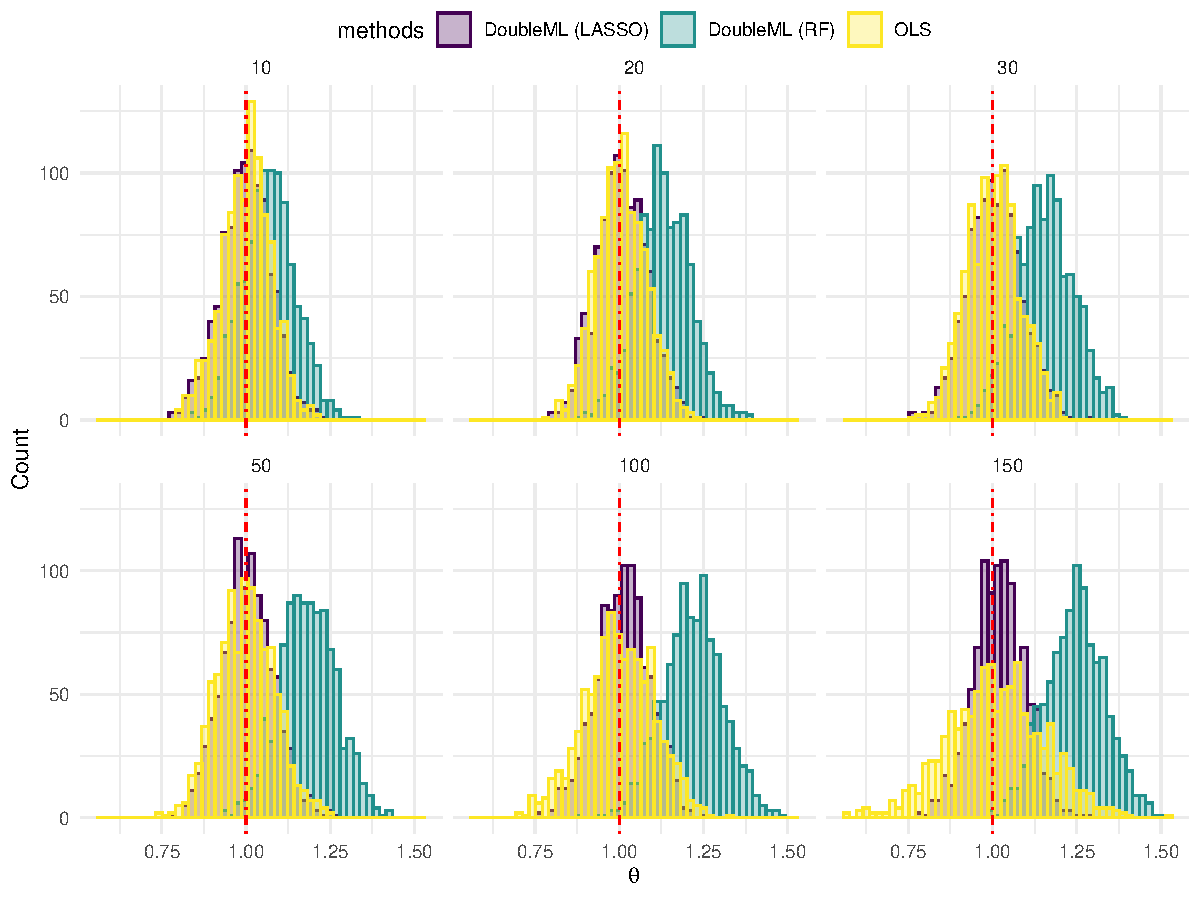
\includegraphics[width=\linewidth]{figures/simulation-logistic6 (partialling out).pdf}
        \caption{Partialling-Out}
    \end{subfigure}
    \caption{Logistic-like Models for (\ref{eq:logistic-model-2})}
\end{figure}
\clearpage

\section{Indicator Models}

Suppose
\begin{equation}
    \begin{aligned}
        m\left(\mathbf{X}_{i}\right)= & \mathrm{I}_{x_{i,1}>3}+\mathrm{I}_{x_{i,2}>2}+\mathrm{I}_{x_{i,3}>1} \\
        g\left(\mathbf{X}_{i}\right)= & \mathrm{I}_{x_{i,1}>1}+\mathrm{I}_{x_{i,2}>2}+\mathrm{I}_{x_{i,3}>3}
    \end{aligned}
    \label{eq:indicator-model-1}
\end{equation}
or
\begin{equation}
    \begin{aligned}
        m\left(\mathbf{X}_{i}\right)= & \mathrm{I}_{x_{i,1}>3}+\mathrm{I}_{x_{i,2}>2}+\mathrm{I}_{x_{i,3}>1}+\mathrm{I}_{x_{i,4}>-1}+\mathrm{I}_{x_{i,5}>-2}+\mathrm{I}_{x_{i,6}>-3}+\mathrm{I}_{x_{i,1}x_{i,6}>0}+\mathrm{I}_{x_{i,3}x_{i,4}>1} \\
        g\left(\mathbf{X}_{i}\right)= & \mathrm{I}_{x_{i,1}>1}+\mathrm{I}_{x_{i,2}>2}+\mathrm{I}_{x_{i,3}>3}+\mathrm{I}_{x_{i,4}>-3}+\mathrm{I}_{x_{i,5}>-2}+\mathrm{I}_{x_{i,6}>-1}+\mathrm{I}_{x_{i,1}x_{i,6}>2}+\mathrm{I}_{x_{i,3}x_{i,4}>-1}
        \label{eq:indicator-model-2}
    \end{aligned}
\end{equation}
where
\begin{equation*}
    \mathbf{X}_{i}\sim N\left(\boldsymbol{0},\mathrm{I}_{p}\right)\text{ and }U_{i},V_{i}\sim N\left(0,1\right),\quad i=1,2,\ldots,n.
\end{equation*}

\begin{figure}[htp]
    \centering
    \begin{subfigure}{.41\textwidth}
        \centering
        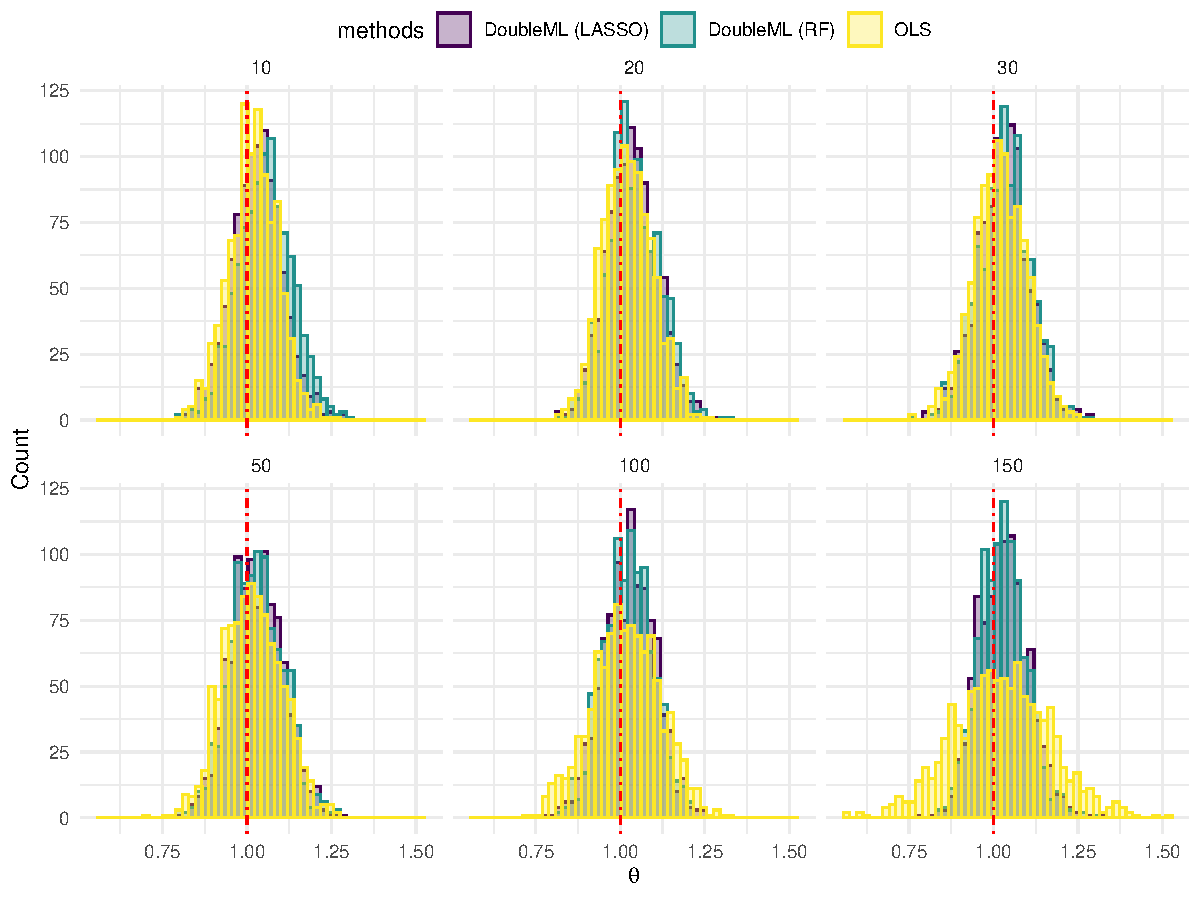
\includegraphics[width=\linewidth]{figures/simulation-indicator3 (IV-type).pdf}
        \caption{IV-type}
    \end{subfigure}
    \begin{subfigure}{.41\textwidth}
        \centering
        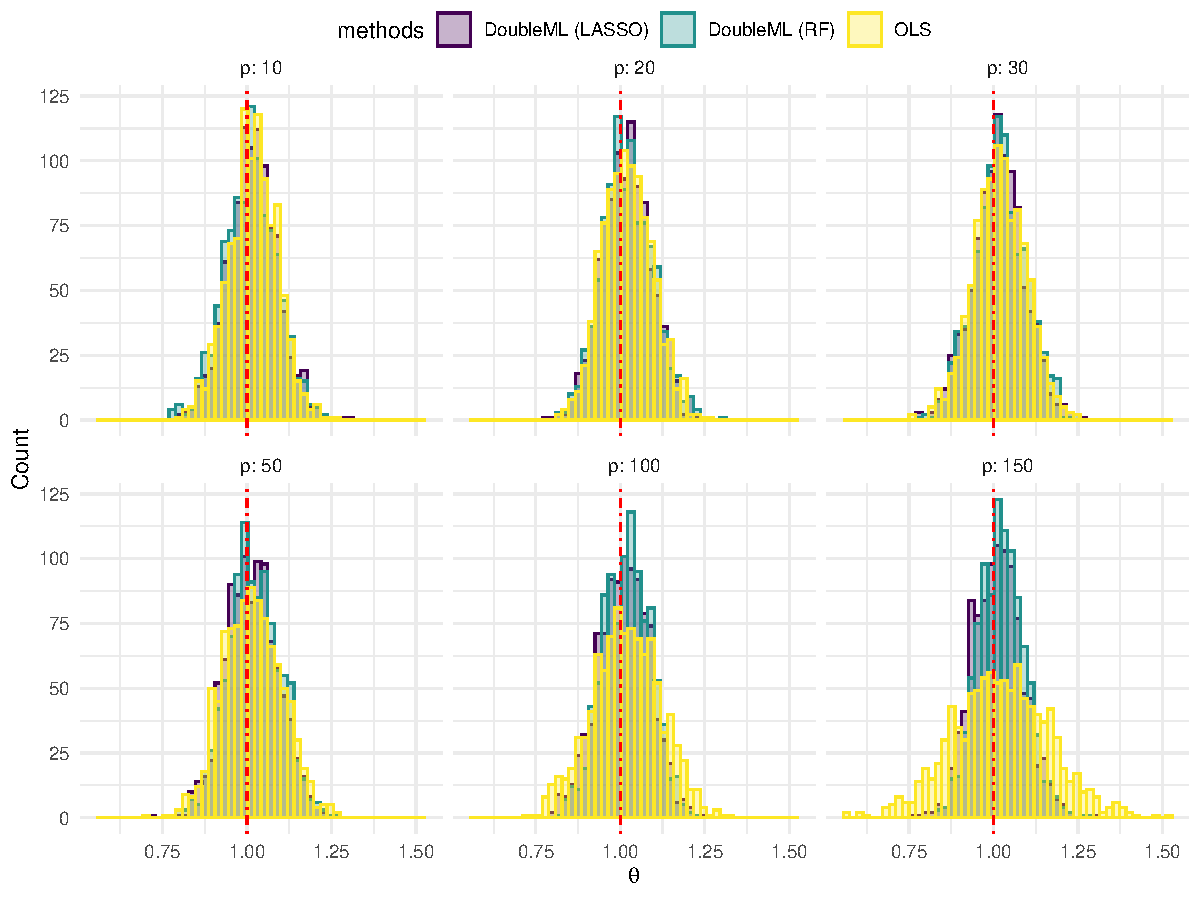
\includegraphics[width=\linewidth]{figures/simulation-indicator3 (partialling out).pdf}
        \caption{Partialling-Out}
    \end{subfigure}
    \caption{Indicator Models for (\ref{eq:indicator-model-1})}
\end{figure}

\begin{figure}[htp]
    \centering
    \begin{subfigure}{.41\textwidth}
        \centering
        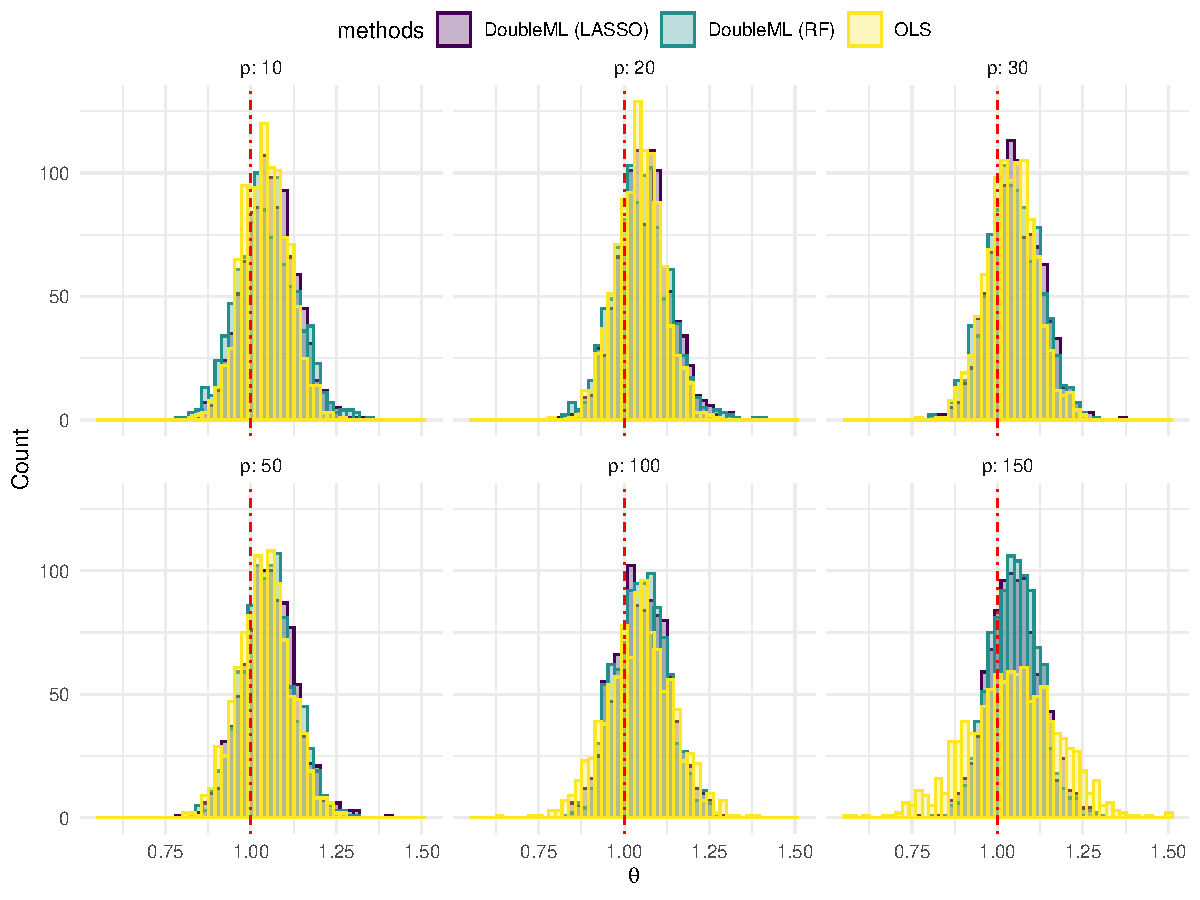
\includegraphics[width=\linewidth]{figures/simulation-indicator6 (IV-type).pdf}
        \caption{IV-type}
    \end{subfigure}
    \begin{subfigure}{.41\textwidth}
        \centering
        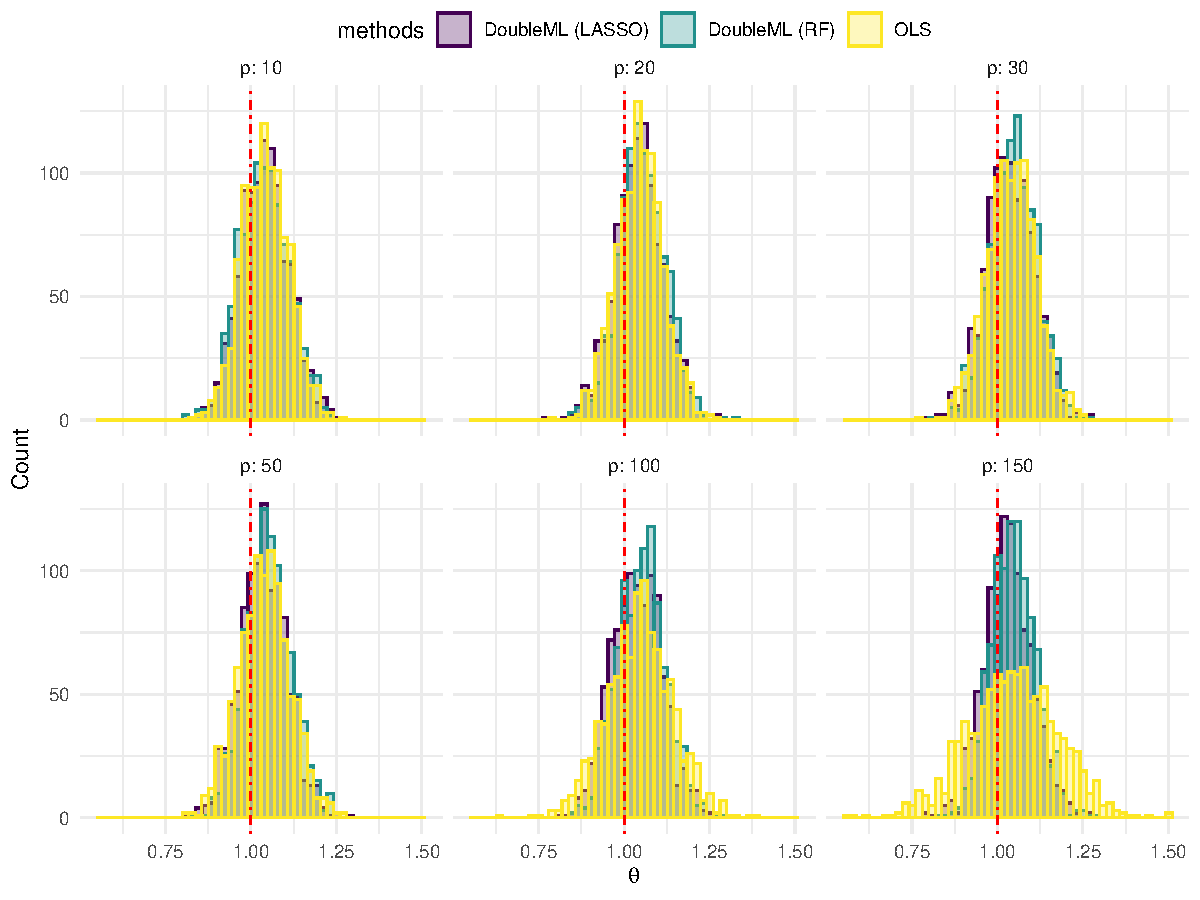
\includegraphics[width=\linewidth]{figures/simulation-indicator6 (partialling out).pdf}
        \caption{Partialling-Out}
    \end{subfigure}
    \caption{Indicator Models for (\ref{eq:indicator-model-2})}
\end{figure}
\clearpage

\end{document}